% !TeX root = ../main.tex

\chapter{Results}\label{chapter:results}

This chapter presents the experimental results of our investigation into enhancing intraoperative registration with Neural Radiance Fields through different loss functions. We begin with a description of our nerfstudio-based implementation, followed by a comprehensive evaluation of different loss functions and their impact on registration performance.

\section{NeRF-Based Registration Implementation}

One of the primary contributions of this work is the development of a nerfstudio-based implementation of neural registration that is agnostic to the specific NeRF model architecture (e.g., vanilla NeRF, InstantNGP). This implementation leverages finite differences to compute gradients and provides a flexible framework for experimenting with different loss functions.

\subsection{Optimization Strategy}

Our implementation follows an inverse neural rendering approach inspired by iNeRF \parencite{yen2020inerf}. The key steps in our optimization strategy are as follows:

\begin{enumerate}
    \item Start with an initial camera pose in 3D NeRF space, represented as a transformation matrix.
    
    \item Render a snapshot from the pre-trained NeRF at the current pose.
    
    \item Calculate the error between the rendered image and the target image using the selected loss function.
    
    \item Update the camera pose through optimization to minimize this error.
    
    \item Repeat steps 2-4 until convergence or a maximum number of iterations is reached.
\end{enumerate}

To overcome challenges with gradient flow disconnection in the rendering pipeline, we implemented a finite differences approach for gradient computation. This approach, while computationally more intensive than direct backpropagation, provides stable and reliable gradients for pose optimization.

\section{Loss Function Evaluation}

We evaluated the performance of five different loss functions in the context of NeRF-based registration:

\begin{itemize}
    \item L1 Loss (Mean Absolute Error)
    \item L2 Loss (Mean Squared Error)
    \item Structural Similarity Index Loss (SSIM)
    \item Normalized Cross-Correlation Loss (NCC)
    \item Mutual Information Loss (MI)
\end{itemize}

Our evaluation focused on convergence behavior, stability, and final registration accuracy across multiple starting positions.

\subsection{Experimental Setup}

To ensure controlled and reproducible results, we established the following experimental setup:

\begin{itemize}
    \item All experiments were limited to 50 iterations
    \item AdamW optimizer with a learning rate of 0.01
    \item 10 different starting points with the same target image
    \item Both target and rendered images sourced from the same NeRF model
    \item Batch size of 12 for finite differences gradient computation
\end{itemize}

\subsection{Convergence Behavior}

Table~\ref{tab:loss_convergence} summarizes the average convergence performance of different loss functions in our experiments.

\begin{table}[htpb]
  \caption[Convergence performance of different loss functions]{Average convergence performance of different loss functions.}\label{tab:loss_convergence}
  \centering
  \begin{tabular}{l c c}
    \toprule
      Loss Function & Average Best Loss Iteration & Average Time Elapsed (s) \\
    \midrule
      L1 & 39 & 621 \\
      L2 & 47 & 624 \\
      Structural Similarity Index & 49 & 626 \\
      Normalized Cross-Correlation & 44 & 621 \\
      Mutual Information & 42 & 621 \\
    \bottomrule
  \end{tabular}
\end{table}

Our results indicate that L1 loss converges more quickly on average compared to other loss functions, reaching its best loss value around iteration 39. In contrast, SSIM requires almost the full 50 iterations before converging to its best value.

Figure~\ref{fig:loss_convergence} illustrates the typical convergence behavior of different loss functions during the registration optimization process.

\begin{figure}[htpb]
  \centering
  % Add actual figure in the implementation
  \caption[Convergence behavior of different loss functions]{Convergence behavior of different loss functions during registration optimization. The plot shows the evolution of loss as a function of optimization iterations.}
  \label{fig:loss_convergence}
\end{figure}

\subsection{Qualitative Analysis}

Our qualitative analysis of the optimization trajectories revealed several interesting patterns:

\begin{itemize}
    \item L1 and L2 losses tend to follow smoother, more direct paths during optimization, with L1 generally converging faster.
    
    \item Mutual Information and Normalized Cross-Correlation losses exhibit more "exploratory" behavior in early iterations, with more pronounced oscillations in the optimization path.
    
    \item SSIM demonstrates slower initial progress but continues to improve throughout the optimization process.
    
    \item MI and NCC appear to be more robust to NeRF rendering artifacts, potentially making them more suitable for cross-modal scenarios.
\end{itemize}

\subsection{Registration Accuracy and Stability}

While all loss functions eventually achieved visually satisfactory registration results, our observations suggest differences in their stability and robustness:

\begin{itemize}
    \item L1 loss provides the fastest convergence while maintaining good stability.
    
    \item MI and NCC show greater resilience to local optima, potentially offering advantages in real-world scenarios with imperfect NeRF representations.
    
    \item SSIM focuses more on structural alignment at multiple scales, which may be beneficial for preserving anatomical structure correspondence.
\end{itemize}

\section{L1 Loss Performance}

The L1 loss (Mean Absolute Error) demonstrated the fastest average convergence among the tested loss functions. Figure~\ref{fig:l1_overlay} shows an overlay of the final registered image on the target for a representative L1 optimization run.

\begin{figure}[htpb]
  \centering
  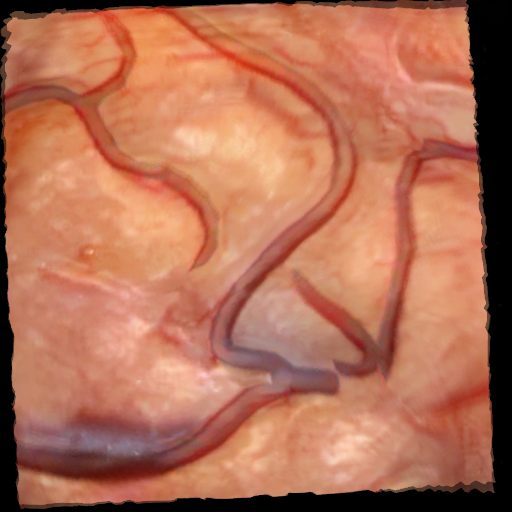
\includegraphics[scale=0.5]{figures/l1/alignment_overlay.png}
  \caption[Registration result with L1 loss]{Overlay of the final registered image on the target image using L1 loss.}
  \label{fig:l1_overlay}
\end{figure}

Figure~\ref{fig:l1_history} shows the corresponding loss history for this optimization run.

\begin{figure}[htpb]
  \centering
  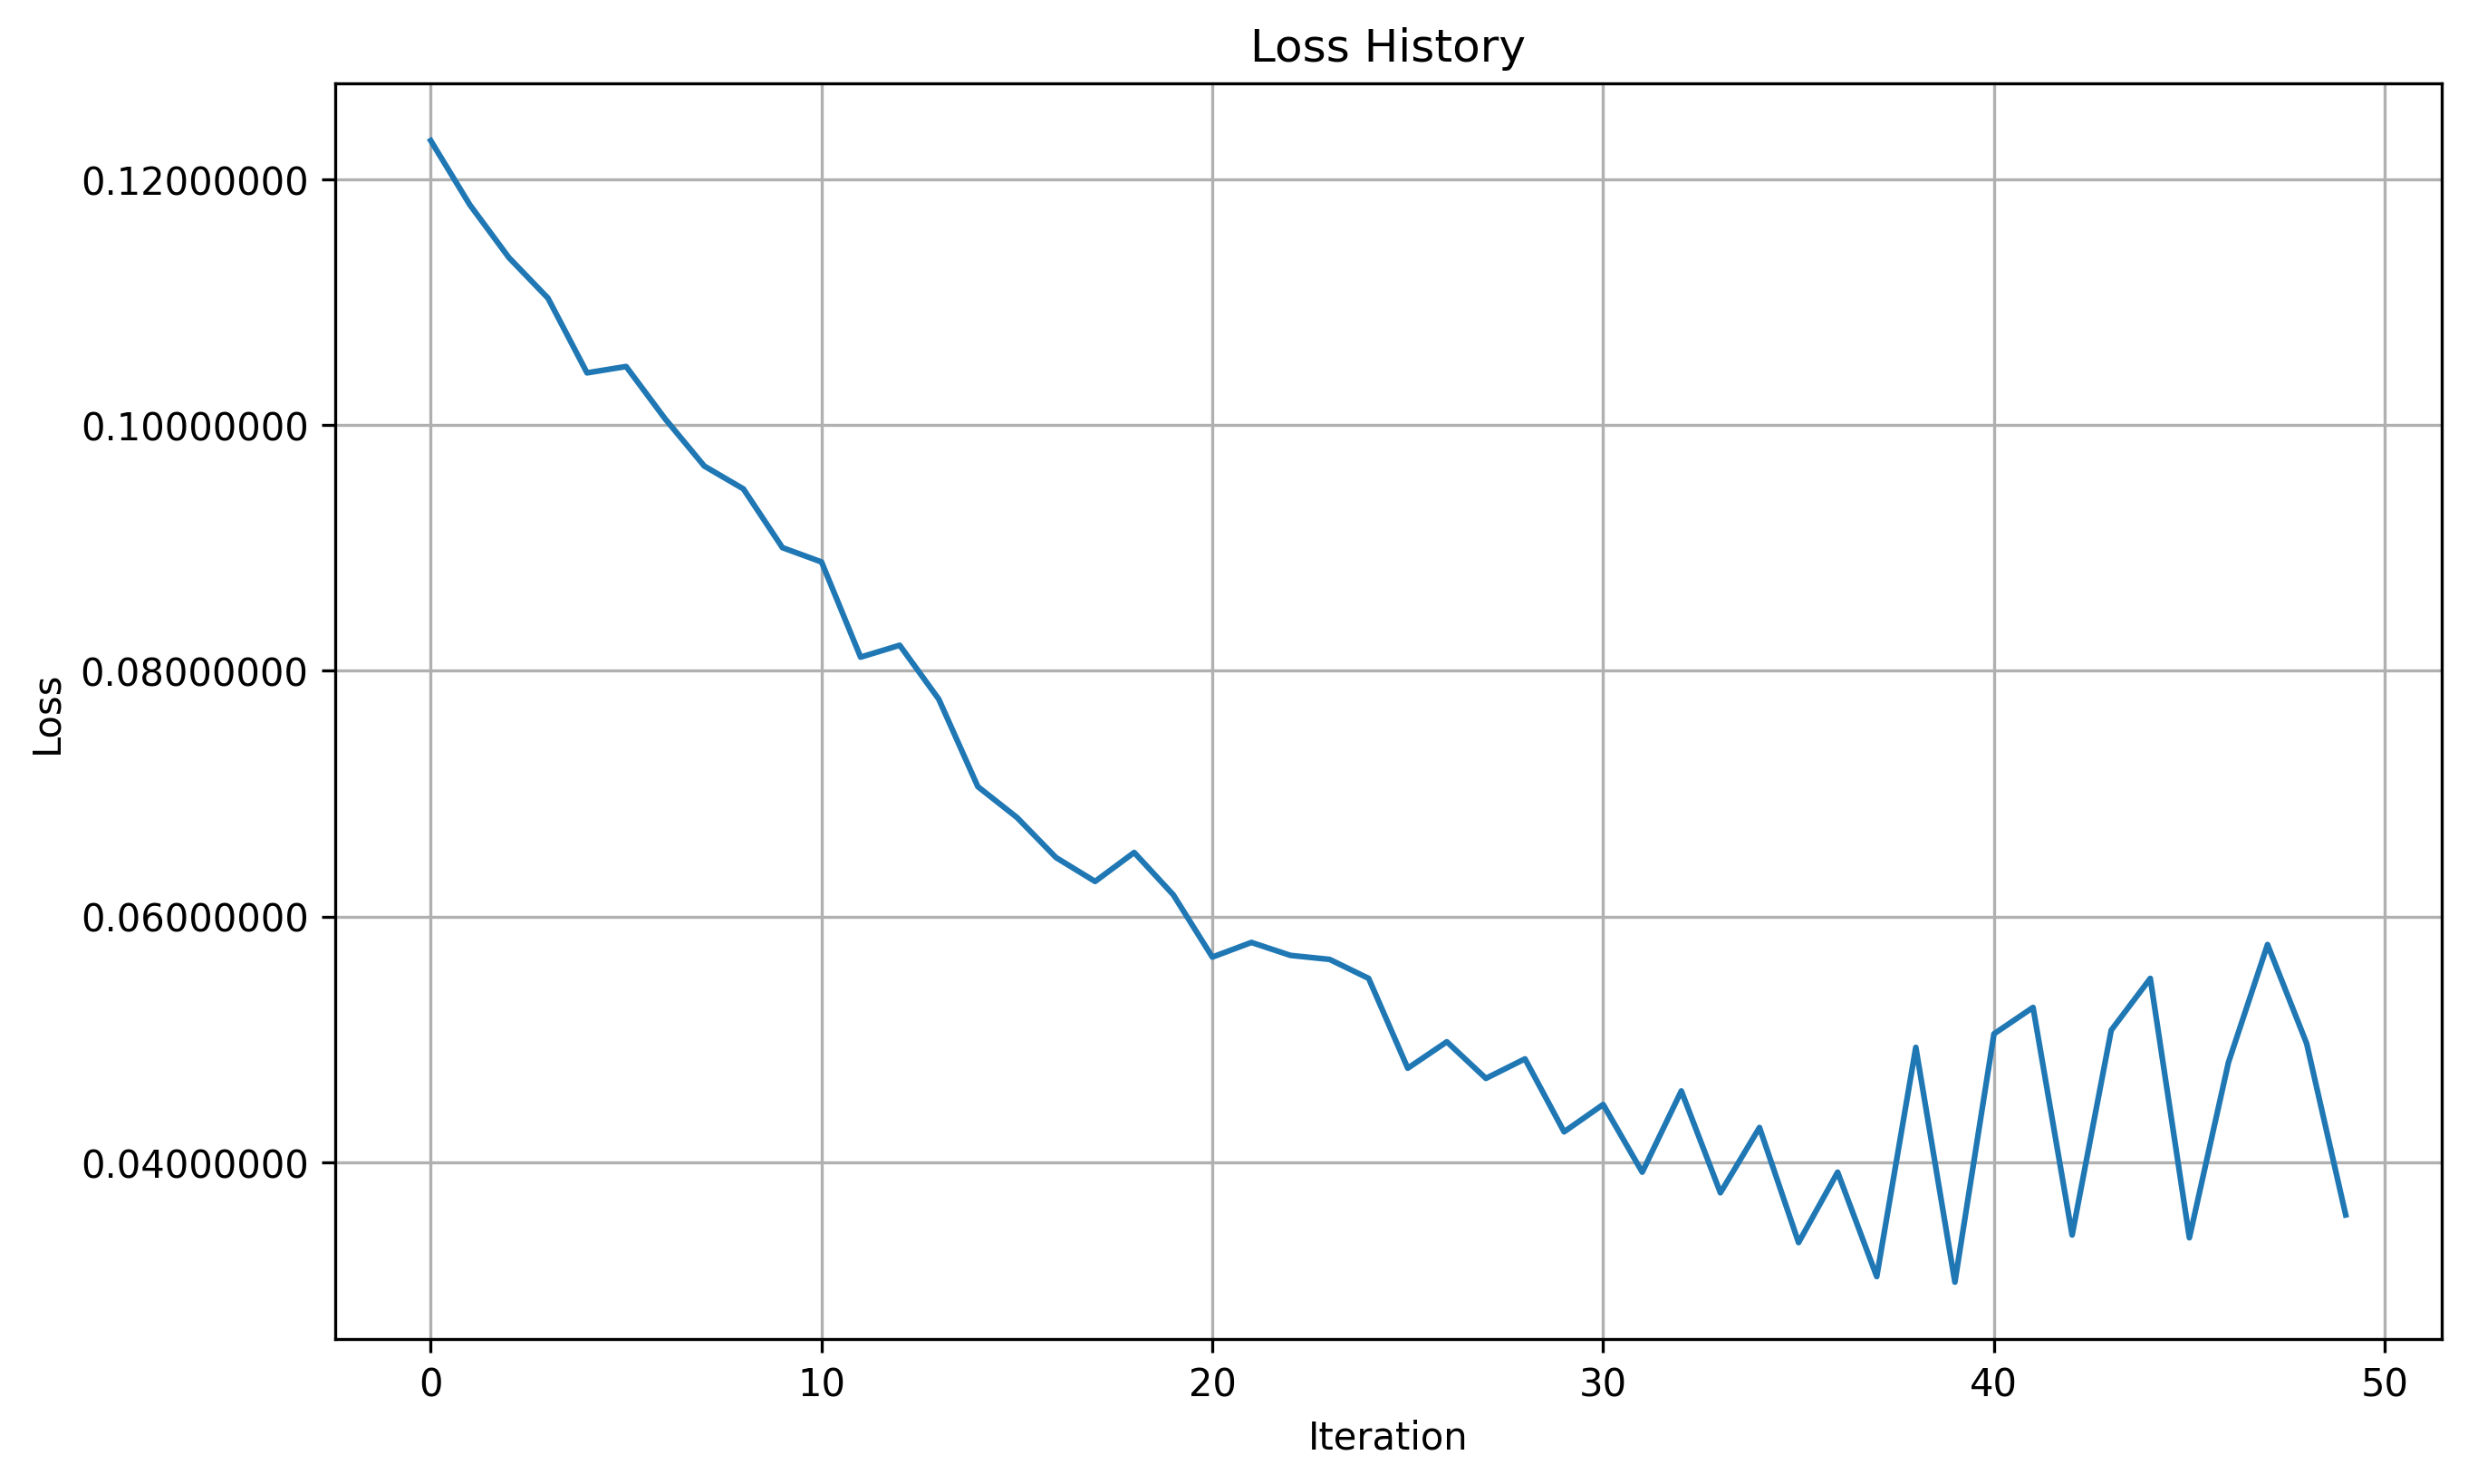
\includegraphics[scale=0.65]{figures/l1/loss_history.png}
  \caption[Loss history for L1 optimization]{Loss history for registration optimization using L1 loss.}
  \label{fig:l1_history}
\end{figure}

The L1 loss function achieved consistent and rapid convergence, reaching its best value at an average of 39 iterations. This suggests that L1 loss may be preferable in scenarios where computational efficiency is a priority.

\section{L2 Loss Performance}

The L2 loss (Mean Squared Error) is the most commonly used loss function in NeRF-based registration approaches, including the original iNeRF implementation. Figure~\ref{fig:l2_overlay} shows an overlay of the final registered image on the target for a representative L2 optimization run.

\begin{figure}[H]
  \centering
  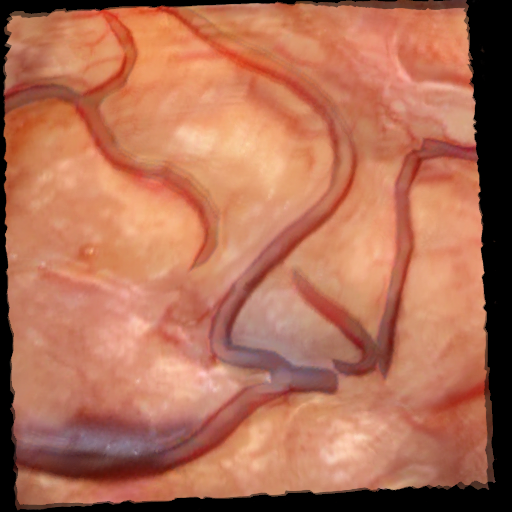
\includegraphics[scale=0.5]{figures/l2/alignment_overlay.png}
  \caption[Registration result with L2 loss]{Overlay of the final registered image on the target image using L2 loss.}
  \label{fig:l2_overlay}
\end{figure}

Figure~\ref{fig:l2_history} shows the corresponding loss history for this optimization run.

\begin{figure}[htpb]
  \centering
  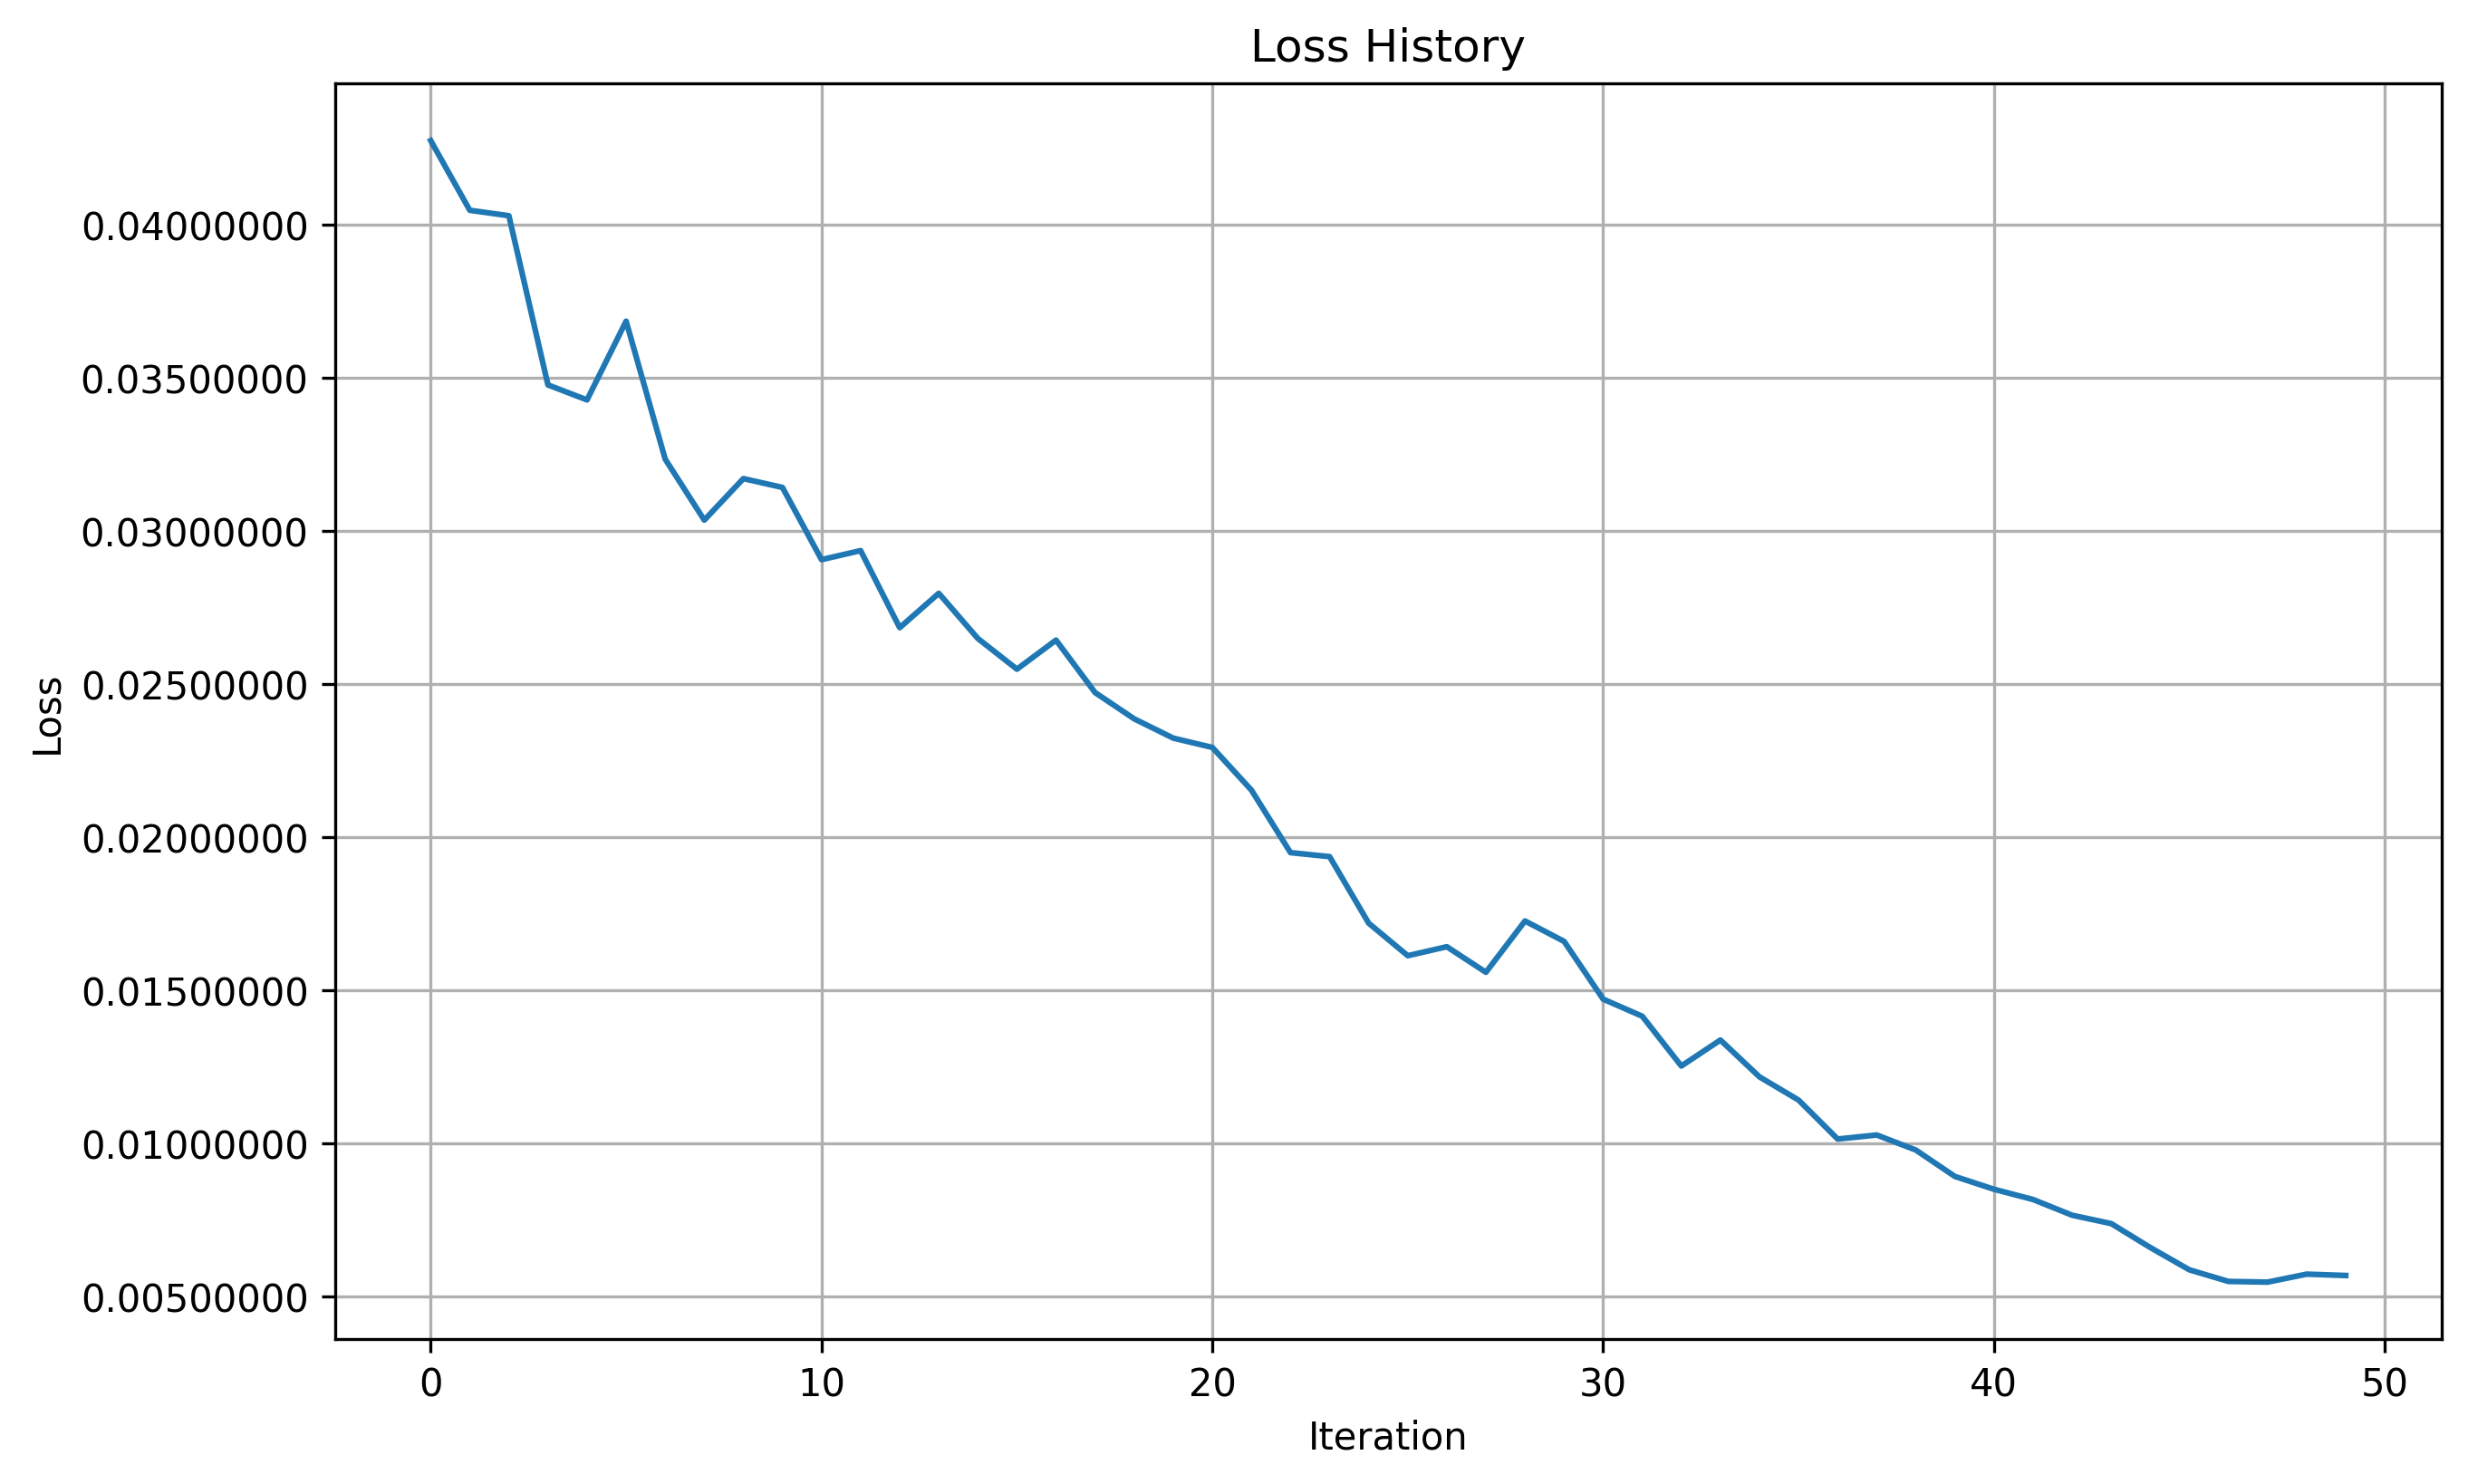
\includegraphics[scale=0.65]{figures/l2/loss_history.png}
  \caption[Loss history for L2 optimization]{Loss history for registration optimization using L2 loss.}
  \label{fig:l2_history}
\end{figure}

The L2 loss required more iterations to converge compared to L1, with an average best loss occurring at iteration 47. This suggests that while L2 can achieve high-quality registration, it may require more computational resources to reach convergence.

\section{Structural Similarity Index Loss Performance}

The Structural Similarity Index (SSIM) loss focuses on preserving structural information rather than pixel-wise differences. Figure~\ref{fig:ssim_overlay} shows an overlay of the final registered image on the target for a representative SSIM optimization run.

\begin{figure}[htpb]
  \centering
  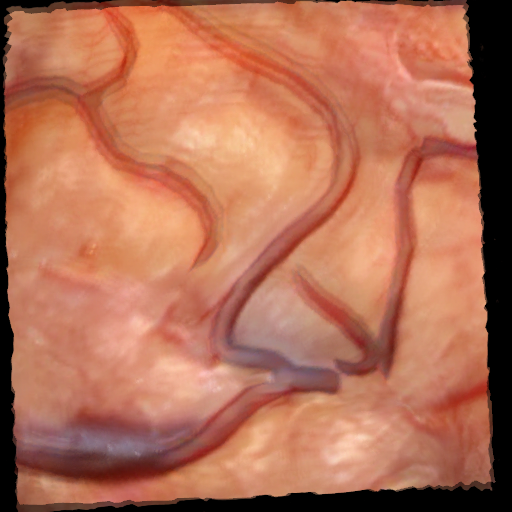
\includegraphics[scale=0.5]{figures/ssim/alignment_overlay.png}
  \caption[Registration result with SSIM loss]{Overlay of the final registered image on the target image using SSIM loss.}
  \label{fig:ssim_overlay}
\end{figure}

Figure~\ref{fig:ssim_history} shows the corresponding loss history for this optimization run.

\begin{figure}[htpb]
  \centering
  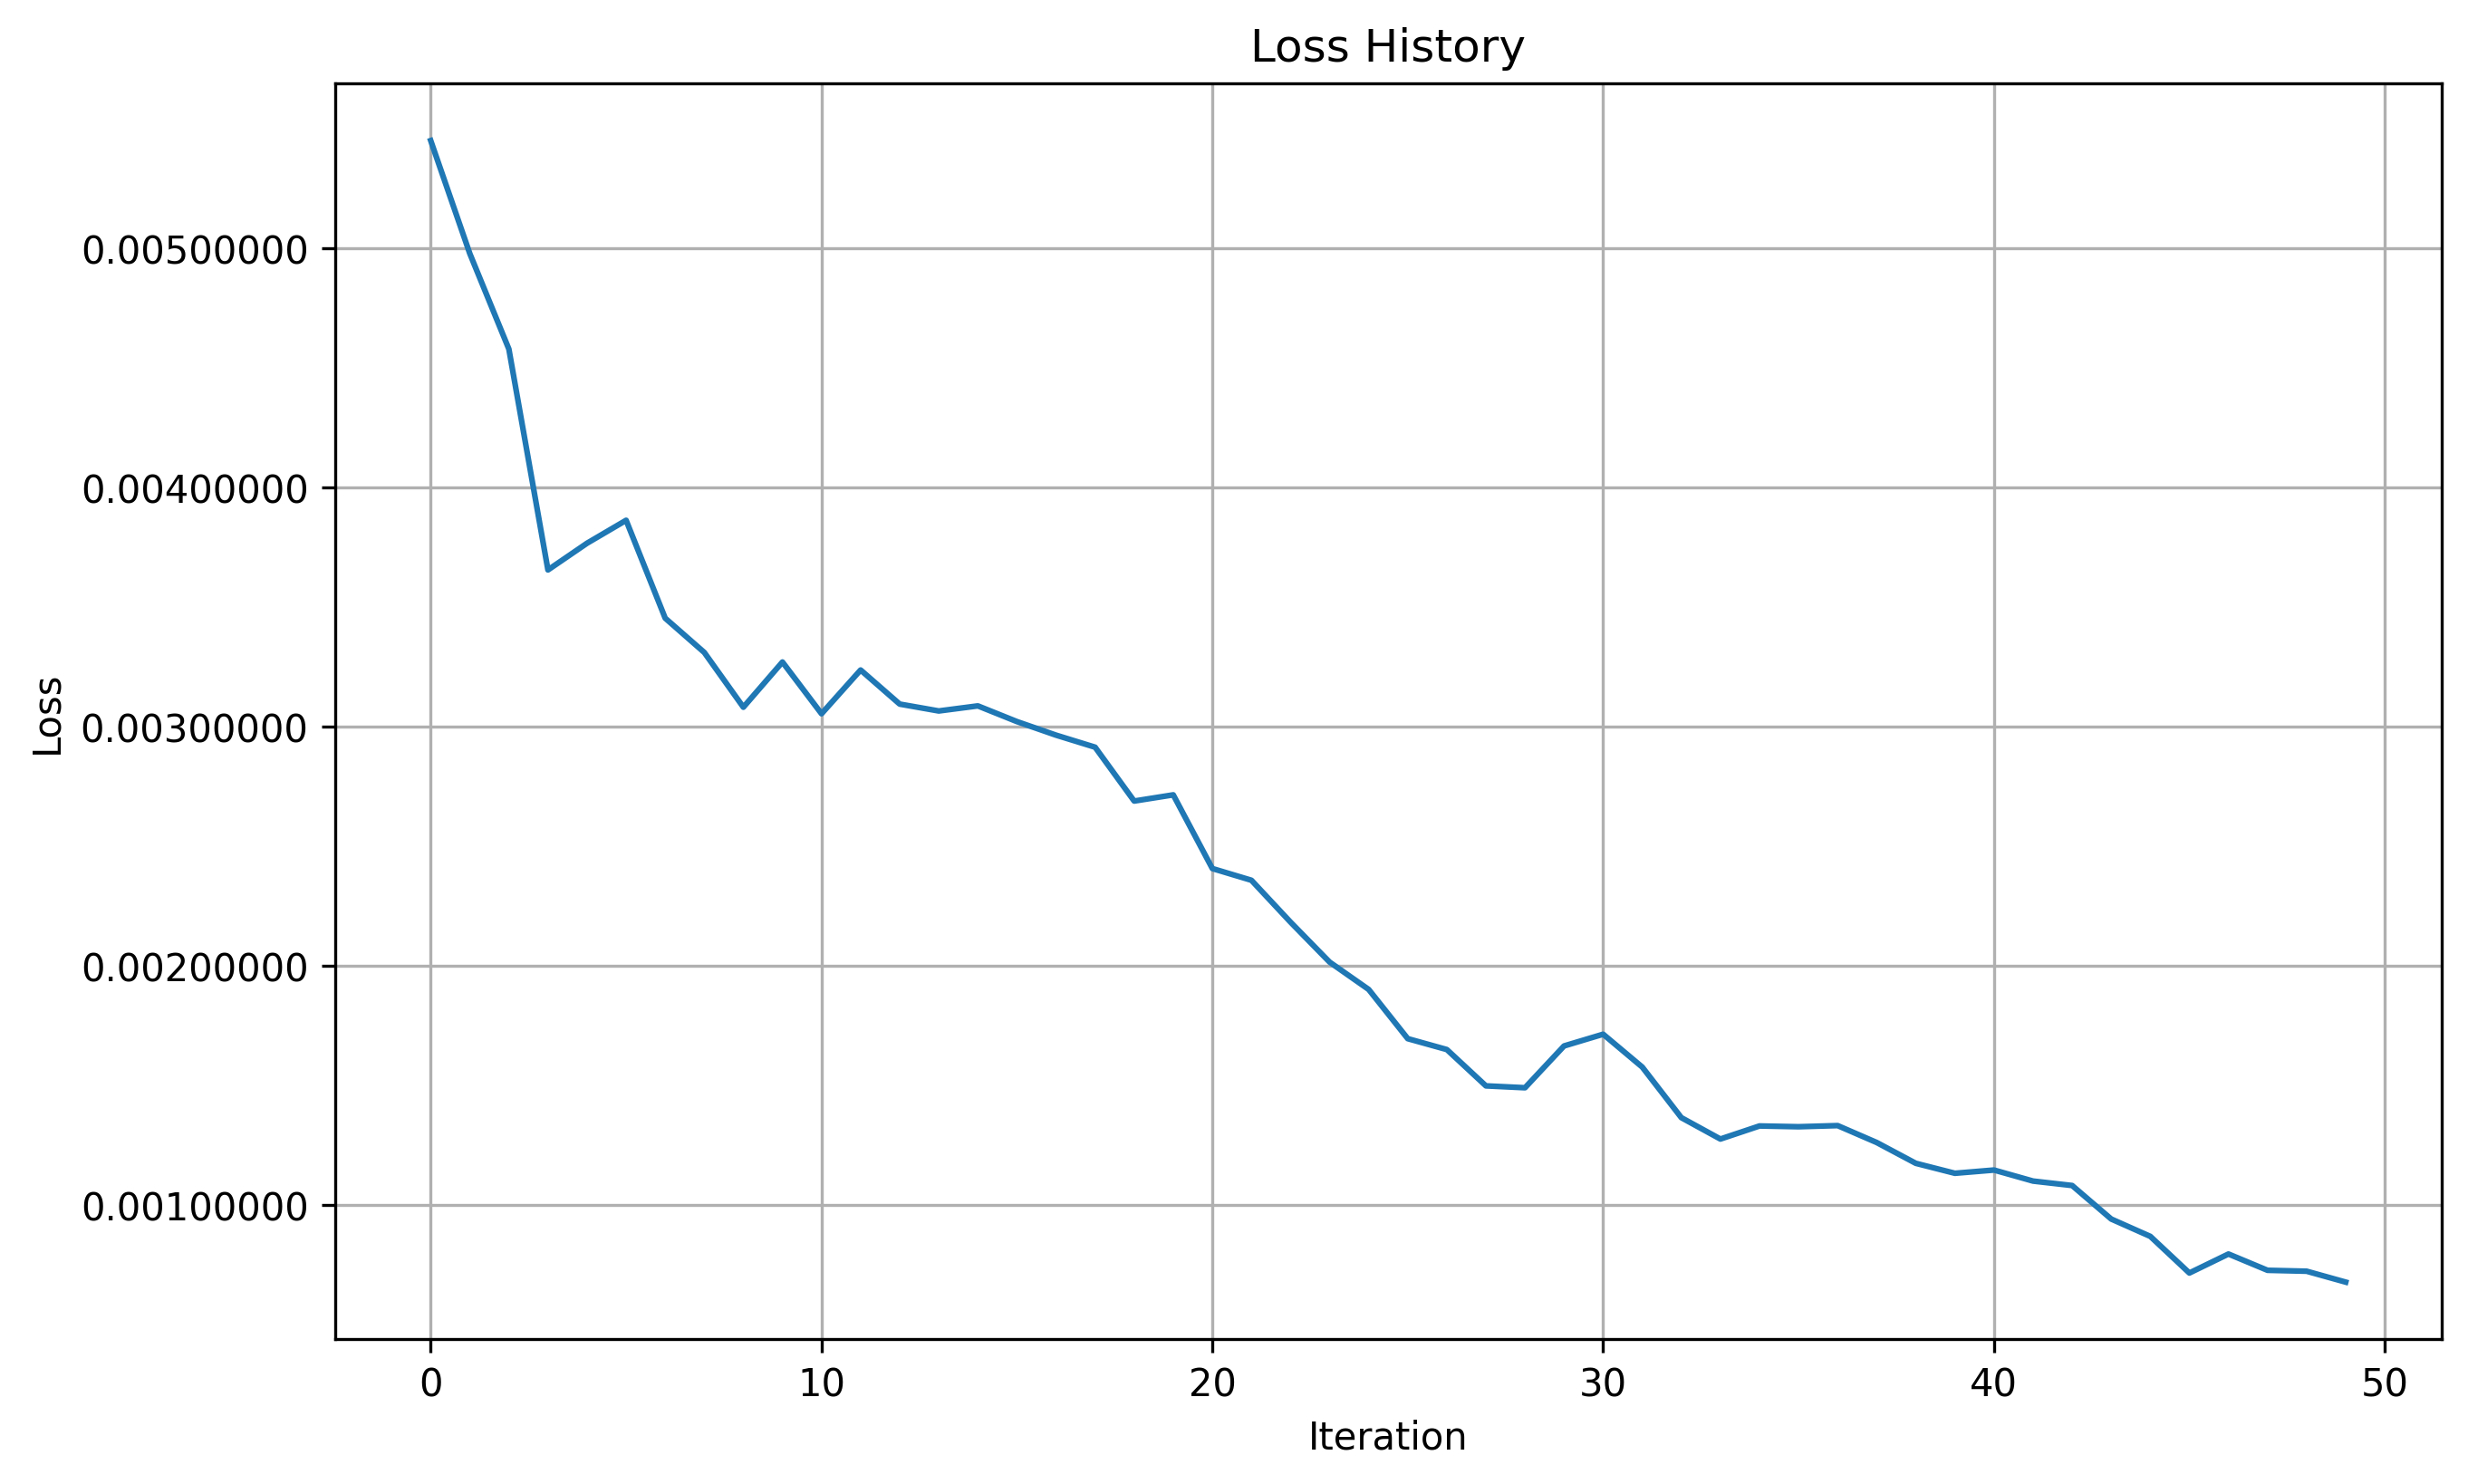
\includegraphics[scale=0.65]{figures/ssim/loss_history.png}
  \caption[Loss history for SSIM optimization]{Loss history for registration optimization using SSIM loss.}
  \label{fig:ssim_history}
\end{figure}

The SSIM loss function required the most iterations to reach its best value, with an average of 49 iterations. This suggests that while SSIM can provide high-quality registration with emphasis on structural correspondence, it may require more computational time to converge fully.

\section{Normalized Cross-Correlation Loss Performance}

Normalized Cross-Correlation (NCC) is often used in multi-modal registration scenarios due to its invariance to linear intensity changes. Figure~\ref{fig:ncc_overlay} shows an overlay of the final registered image on the target for a representative NCC optimization run.

\begin{figure}[htpb]
  \centering
  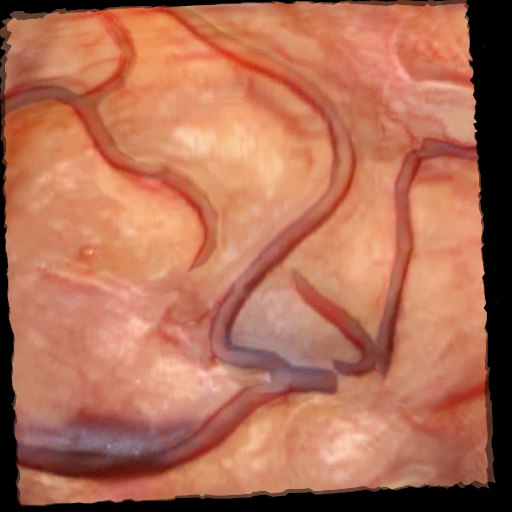
\includegraphics[scale=0.5]{figures/ncc/alignment_overlay.png}
  \caption[Registration result with NCC loss]{Overlay of the final registered image on the target image using NCC loss.}
  \label{fig:ncc_overlay}
\end{figure}

Figure~\ref{fig:ncc_history} shows the corresponding loss history for this optimization run.

\begin{figure}[htpb]
  \centering
  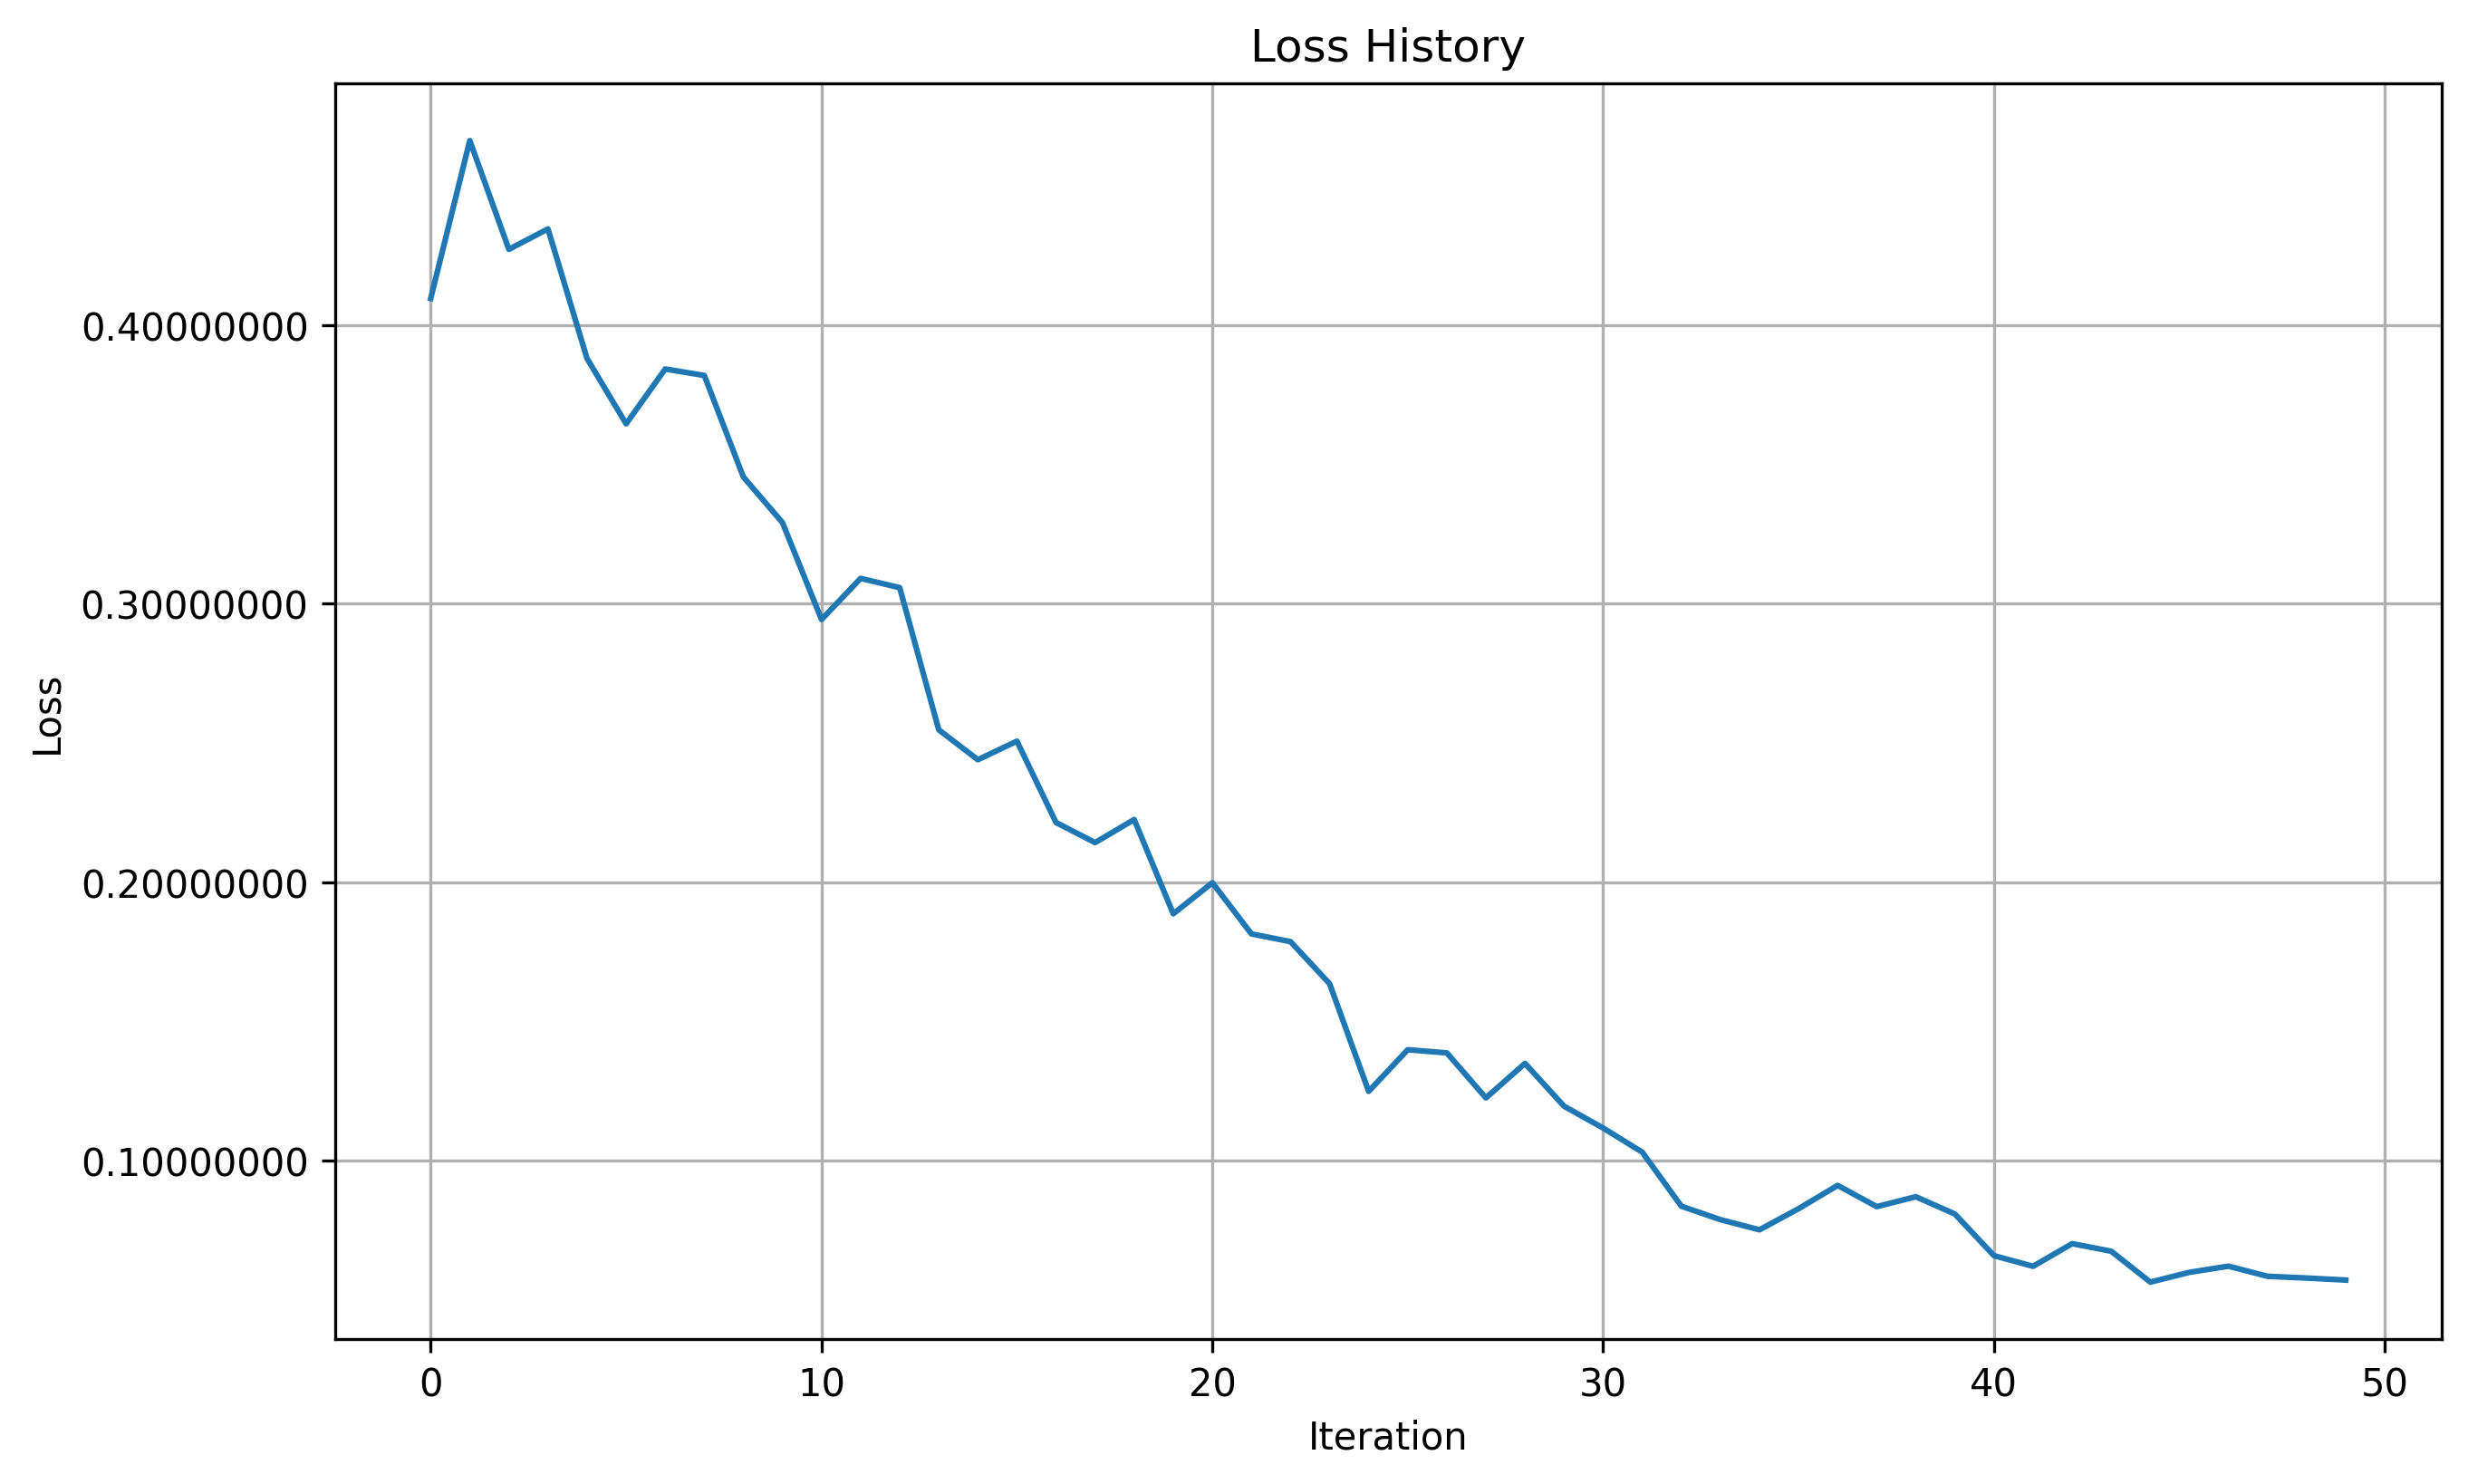
\includegraphics[scale=0.65]{figures/ncc/loss_history.png}
  \caption[Loss history for NCC optimization]{Loss history for registration optimization using NCC loss.}
  \label{fig:ncc_history}
\end{figure}

The NCC loss function demonstrated moderate convergence speed, with its best value occurring at an average of 44 iterations. While slightly slower than L1, NCC showed good stability and robustness to intensity variations.

\section{Mutual Information Loss Performance}

Mutual Information (MI) is a widely used similarity measure for multi-modal registration. Figure~\ref{fig:mi_overlay} shows an overlay of the final registered image on the target for a representative MI optimization run.

\begin{figure}[htpb]
  \centering
  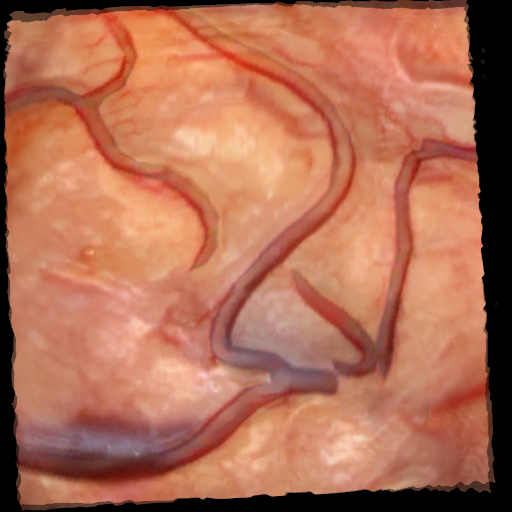
\includegraphics[scale=0.5]{figures/mi/alignment_overlay.png}
  \caption[Registration result with MI loss]{Overlay of the final registered image on the target image using MI loss.}
  \label{fig:mi_overlay}
\end{figure}

Figure~\ref{fig:mi_history} shows the corresponding loss history for this optimization run.

\begin{figure}[htpb]
  \centering
  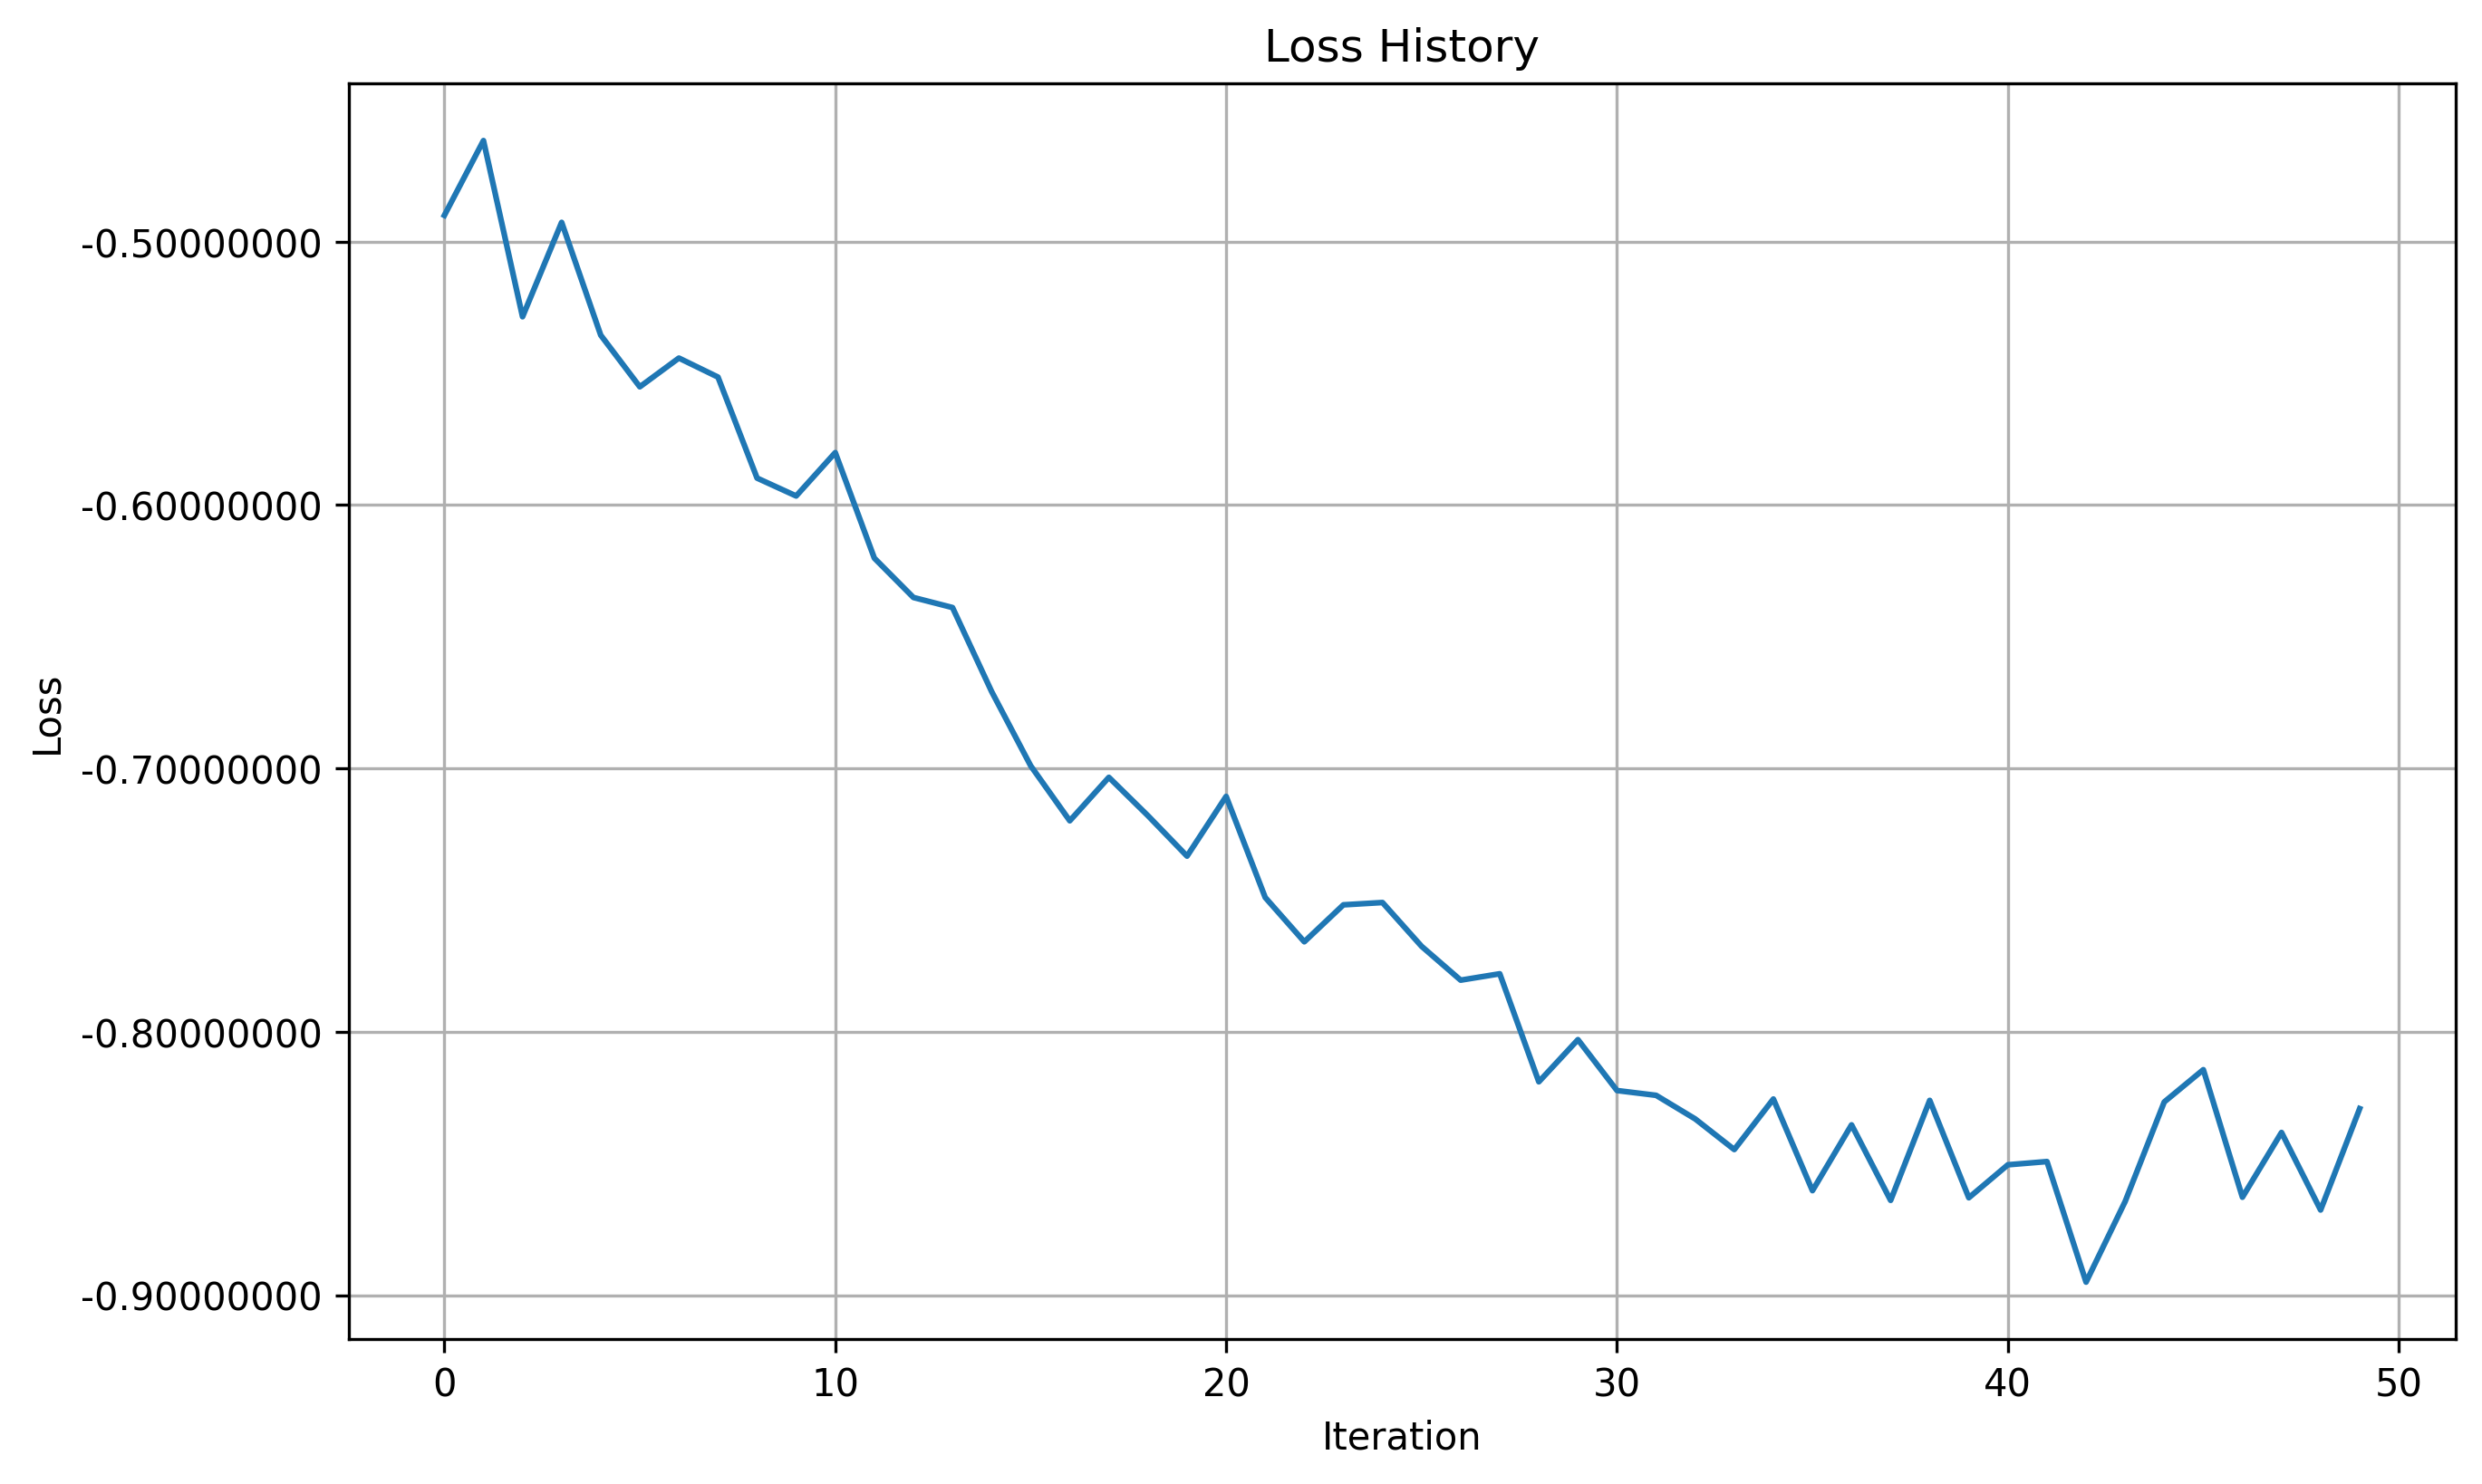
\includegraphics[scale=0.65]{figures/mi/loss_history.png}
  \caption[Loss history for MI optimization]{Loss history for registration optimization using MI loss.}
  \label{fig:mi_history}
\end{figure}

The MI loss function reached its best value at an average of 42 iterations, placing it between L1 and NCC in terms of convergence speed. The more exploratory optimization path of MI may contribute to its robustness in complex registration scenarios.

\section{Limitations and Challenges}

Our implementation and evaluation encountered several limitations and challenges that should be considered:

\begin{itemize}
    \item The use of finite differences for gradient computation, while effective, is computationally more expensive than direct backpropagation.
    
    \item Our experiments assumed perfect NeRF representation of the target object, which is a simplification of real-world scenarios where appearance and lighting variations are significant.
    
    \item The computational cost of registration (averaging around 621-626 seconds for 50 iterations) may be challenging for real-time clinical applications.
    
    \item Our evaluation was limited to a specific set of hyperparameters (learning rate, optimizer, batch size) and may not reflect performance under different conditions.
\end{itemize}

\section{Summary of Findings}

Based on our comprehensive evaluation, we summarize the key findings of our study:

\begin{enumerate}
    \item Our nerfstudio-based implementation provides a flexible framework for experimenting with different loss functions in NeRF-based registration, independent of the specific NeRF architecture.
    
    \item L1 loss demonstrates the fastest convergence among the tested loss functions, making it potentially suitable for time-sensitive applications.
    
    \item Mutual Information and Normalized Cross-Correlation losses exhibit more exploratory behavior during optimization and appear more robust to NeRF rendering artifacts.
    
    \item SSIM loss shows slower convergence but maintains focus on structural correspondence, which may be beneficial for preserving anatomical structures.
    
    \item All five loss functions eventually achieve visually satisfactory registration, suggesting that the choice of loss function may depend on specific application requirements such as speed, robustness, or structural preservation.
\end{enumerate}

These results highlight the importance of loss function selection in NeRF-based registration and provide a foundation for future work in this area. 